\documentclass[tikz,convert={outfile=\jobname.svg}]{standalone}
\begin{document}
   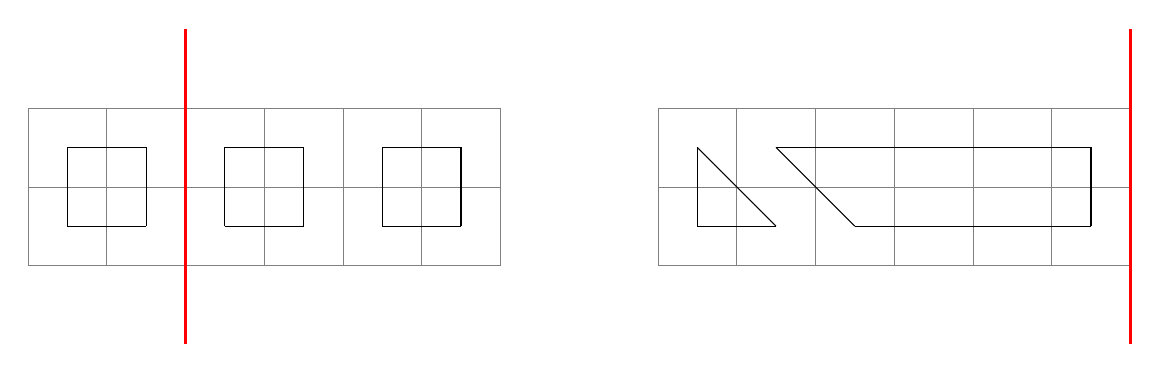
\begin{tikzpicture}
      \foreach \i in {0, ..., 6} {
         \draw[very thin, gray] (\i, 0) -- (\i, 2);
      }
      \foreach \i in {0, 1, 2} {
         \draw[very thin, gray] (0, \i) -- (6, \i);
      }
      \foreach \i in {0.5, 2.5, 4.5} {
         \draw (\i, 0.5) -- (\i+1, 0.5);
         \draw (\i, 1.5) -- (\i+1, 1.5);
      }
      \foreach \i in {0.5, ..., 5.5} {
         \draw (\i, 0.5) -- (\i, 1.5);
      }
      \draw[very thick, red] (2, -1) -- (2, 3);
      \foreach \i in {8, ..., 14} {
         \draw[very thin, gray] (\i, 0) -- (\i, 2);
      }
      \foreach \i in {0, 1, 2} {
         \draw[very thin, gray] (8, \i) -- (14, \i);
      }
      \draw (8.5, 0.5) -- (9.5, 0.5);
      \draw (9.5, 0.5) -- (8.5, 1.5);
      \draw (8.5, 1.5) -- (8.5, 0.5);
      \draw (10.5, 0.5) -- (13.5, 0.5);
      \draw (13.5, 0.5) -- (13.5, 1.5);
      \draw (13.5, 1.5) -- (9.5, 1.5);
      \draw (9.5, 1.5) -- (10.5, 0.5);
      \draw[very thick, red] (14, -1) -- (14, 3);
   \end{tikzpicture}
\end{document}
